
\documentclass[10pt,a4paper]{article}
\usepackage[utf8]{inputenc}
\usepackage[T1]{fontenc}
\usepackage{geometry}
\geometry{margin=1in}
\usepackage{graphicx}
\usepackage{parskip}
\usepackage{titlesec}
\usepackage{xcolor}
\usepackage{enumitem}
\usepackage{hyperref}
\usepackage{fontawesome5}
\usepackage{setspace}
\usepackage{titling}

% Color settings
\definecolor{primary}{RGB}{0, 79, 144}
\definecolor{accent}{RGB}{50, 50, 50}

% Section formatting
\titleformat{\section}
  {\Large\bfseries\color{primary}}{}{0em}{}
\titleformat{\subsection}[runin]
  {\bfseries\color{primary}}{}{0em}{}[.]

% Spacing between items
\setlist[itemize]{itemsep=4pt, topsep=4pt}

\hypersetup{
    colorlinks=true,
    linkcolor=primary,
    urlcolor=primary
}

\pagestyle{empty}

\geometry{
  top=1.5cm,
  bottom=1.8cm,
  left=2cm,
  right=2cm
}

\begin{document}

\vspace*{-1cm} % move header block closer to top of page

\noindent
\begin{minipage}[t]{0.65\textwidth}
    \textbf{\fontsize{24pt}{28pt}\selectfont Ryan Matthews}\\[0.2cm]
    \href{mailto:ryanjmatthews@gmail.com}{ryanjmatthews@gmail.com} \quad
    \href{https://linkedin.com/in/ryan-j-matthews}{LinkedIn} \quad
    \href{https://github.com/Darainer}{GitHub} \quad +49 176 34599887\\[0.6cm]
    \small
    \setstretch{1.8}
    Engineering leader with over 10 years of experience in automated driving development, delivering business outcomes in both technical and product leadership roles. Passionate about building commercially successful software and AI rich products.
\end{minipage}
\hspace{1.5cm}
\begin{minipage}[t]{0.25\textwidth}
    \raisebox{-\height}{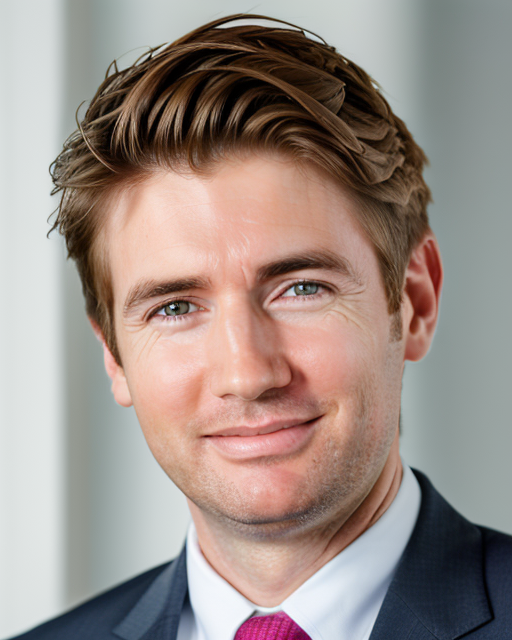
\includegraphics[width=\linewidth]{profile_pic_ryan.png}}
\end{minipage}


\vspace{1.2em}

% Work Experience
\section*{Work Experience}

\subsection*{System Architect ADAS/AD, Luminar, Munich \hfill \textit{Jul 2022 – Present}}
\begin{itemize}
    \item Provide technical direction for the product portfolio, encompassing Software, SoC, and Lidar.
    \item Drove structural changes in software strategy in response to AI-centric sourcing trends.
    \item Designed and socialized a software toolchain to support multidisciplinary development.
\end{itemize}

\subsection*{Product Owner Active Safety, Luminar, Munich \hfill \textit{Sep 2020 – Jun 2022}}
\begin{itemize}
    \item Led NCAP 2023-compliant Lidar-only active safety stack.
    \item Demonstrated solution at \href{https://ces.tech}{CES 2022} and \href{https://ces.tech}{CES 2023}.
    \item Built and mentored a high-performing ADAS development team.
\end{itemize}

\subsection*{Product Owner ADAS, Samsung Electronics, Munich \hfill \textit{Apr 2019 – Sep 2020}}
\begin{itemize}
    \item Led camera-only AEB NCAP 2022+ product development for Samsung SoC.
    \item Directed algorithm development across full software chain.
\end{itemize}

\subsection*{Senior Developer, Zenuity (Volvo / Autoliv JV), Munich \hfill \textit{Mar 2018 – Mar 2019}}
\begin{itemize}
    \item Migrated CI/CD environment and introduced data-driven development.
    \item Enabled daily KPI evaluations via cloud data lake pipeline.
\end{itemize}

\subsection*{Lead Feature Developer, Autoliv Electronics, Munich \hfill \textit{Oct 2016 – Mar 2018}}
\begin{itemize}
    \item Developed tracking/control algorithms for novel camera-only automated driving.
    \item Patented technology, Major camera program wins, successful integration with partners
\end{itemize}

\subsection*{Engineering Consultant, TESIS DYNAware, Munich \hfill \textit{Feb 2011 – Sep 2016}}
\begin{itemize}
    \item Managed projects exceeding \$1M budget with 10-person teams.
    \item Delivered ADAS and ESP algorithms to Tier 1s and German OEMs.
\end{itemize}

\subsection*{Mechatronic Engineer, Australian Submarine Corporation, Perth \hfill \textit{Jan 2007 – Apr 2010}}
\begin{itemize}
    \item Designed and supported submarine control systems on active submarines.
\end{itemize}

\vspace{1.2em}

% Education
\section*{Education}

\textbf{B.Eng (Hons), Mechatronic Engineering}, University of Adelaide \\
\textit{First Class Honours, Dean's List, Aerospace Project Award} \\[4pt]
\textbf{Bachelor of Economics}, University of Adelaide \\
\textit{Major in mathematical modelling and statistics}

\vspace{1.2em}

% Relevant Skills
\section*{Relevant Skills}

\begin{minipage}[t]{0.48\textwidth}
    \textbf{\textcolor{primary}{Software Development}}
    \begin{itemize}
        \item C++
        \item Python
        \item Model based development
    \end{itemize}
\end{minipage}
\hfill
\begin{minipage}[t]{0.48\textwidth}
    \textbf{\textcolor{primary}{Standards / Processes}}
    \begin{itemize}
        \item Functional Safety ISO 26262
        \item SOTIF ISO 21448
        \item AUTOSAR C++ 14
    \end{itemize}
\end{minipage}

\vspace{1.2em}

% Further Education
\section*{Further Education}

\begin{itemize}
    \item \textbf{Nov 2024}: Deep learning Specialization (\href{https://www.deeplearning.ai}{Deeplearning.ai})
    \item \textbf{Sep 2023}: Creative leadership certificate (18 month program \href{https://mvr.de}{mvr.de})
    \item \textbf{July 2022}: Modern C++ training (\href{https://klaus-iglberger.com}{Klaus Iglberger})
    \item \textbf{Apr 2020}: Advanced modern C++ training program (\href{https://nicolaijosuttis.com}{Nicolai Josuttis})
    \item \textbf{Feb 2020}: Professional Scrum Product Owner (\href{https://scrum.org}{scrum.org})
    \item \textbf{Nov 2017}: Certified Scrum Master (\href{https://scrumalliance.org}{Scrum Alliance})
    \item \textbf{Jul 2015}: MathWorks Certified MATLAB Associate (\href{https://www.mathworks.com}{MathWorks})
    \item \textbf{Dec 2014}: Certified Project Management Professional (\href{https://www.pmi.org}{PMP}\textsuperscript{\textregistered})
\end{itemize}

\vspace{1.2em}

% Languages

\section*{Languages}
English (Native), German (Full Professional)

\end{document}
